\documentclass[xcolor*pst]{beamer}
\usetheme{Warsaw}
% Madrid: titre de la diapo en header, nom de la boîte, date et page en footer
% Berlin: liste des sections en header, nom de la boîte en footer

\usefonttheme[onlylarge]{structurebold}
\usecolortheme{orchid}
% orchid: noir sur blanc, headers bleu
% fly: noir sur gris
% albatross: blanc sur bleu
% dove: blanc sur noir
\setbeamerfont*{frametitle}{size=\normalsize,series=\bfseries}
%\setbeamertemplate{navigation symbols}{}

\usepackage[english]{babel}
\usepackage[utf8]{inputenc}
\usepackage[T1]{fontenc}
\usepackage{times}
\usepackage{listings}
\usepackage{relsize}
\usepackage{verbatim}
%\usepackage{hyperref}


\title{}
\author{}
\institute{Catopuma}

\begin{document}

%  \logo{\includegraphics[width=2cm]{ourLogo.png}}
  
  \section{Introduction}

\begin{frame}
\frametitle{Introduction - Objectifs}


\end{frame}



  
  \begin{frame}
    \frametitle*{Table des matières}
    \tableofcontents
  \end{frame}
  
  \section{Python : origine et philosophie}
\subsection{L'origine de Python}
\begin{frame}
  \frametitle{Python - L'origine}
  \begin{columns}
    \begin{column}{5cm}
      \begin{itemize}
        \item<1-> Apparition en 1991
        \item<2-> Créé par Guido van Rossum
        \item<3-> Nombreuses références aux Monty Python
      \end{itemize}
    \end{column}
    \begin{column}{5cm}
      \begin{overprint}
        \includegraphics<2>[scale=0.04]{guido.jpg}
        \includegraphics<3>[scale=0.15]{spam.jpg}
      \end{overprint}
    \end{column}
  \end{columns}
\end{frame}

\subsection{Valeurs et philosophie}
\begin{frame}
\frametitle{Python - Valeurs et philosophie}
  % En fait ici on présente ce qu'on va voir, afin de pouvoir terminer par CQFD!
  \begin{itemize}
    \item<1-> Orienté objet
    %note feth:
    %utilisation souple (programmation impérative, orientée aspect, haut niveau ou bas niveau...)
    \item<2-> Extensible (librairies standard, modules C, C++, \ldots)
    \item<3-> Programmation souple : orientée aspect, haut niveau
    \item<4-> Convergence de l'élégance
  \end{itemize}
\end{frame}

\subsection{La recherche du meilleur chemin}
\begin{frame}
\frametitle{Python - La recherche du meilleur chemin}
  \begin{itemize}
    \item Un travail de recherche via les PEP (Python Enhancement Proposal). Exemples:
    \begin{itemize}
      \item PEP 8: Style Guide for Python Code
      \item PEP 100: Python Unicode Integration
      \item PEP 386: Changing the version comparison module in Distutils
    \end{itemize}
    \pause
    %note feth:
    %mots clefs: efficacité en terme de lisibilité, pythonique, élégance (comme en maths)
    \item Un seul bon moyen de faire, pas de comportement implicite
    \begin{itemize}
      \item Si une déclaration n'est pas assez explicite, on préferera faire échouer la commande
      \item "In the face of ambiguity, refuse the temptation to guess."
    \end{itemize}
    \pause
    \item Si le code n'est pas élégant, c'est qu'il y a une meilleure façon de faire
  \end{itemize}
\end{frame}

\begin{frame}[fragile]
\frametitle{En résumé, la philosophie de Python c'est :}
Tiré de la PEP 20, The Zen of Python :
  \begin{itemize}
    \item Beautiful is better than ugly.
    \item Explicit is better than implicit.
    \item Simple is better than complex.
    \item Complex is better than complicated.
    \item Flat is better than nested.
    \item Sparse is better than dense.
    \item Readability counts.
    \item Special cases aren't special enough to break the rules.
    \item Errors should never pass silently.
    \item In the face of ambiguity, refuse the temptation to guess.
    \item There should be one-- and preferably only one --obvious way to do it.
    \item If the implementation is hard to explain, it's a bad idea.
  \end{itemize}
\end{frame}


\section{IPython, le Python interactif}

\subsection{Présentation}
\begin{frame}[fragile]
  \frametitle{IPython - Présentation}
  \begin{itemize}
    \item Shell python interactif à la façon de \verb=python=
    \item Apporte en plus un certain nombre de fonctionnalités intéressantes
  \end{itemize}
\end{frame}

\subsection{Les fonctionnalités}
\begin{frame}
  \frametitle{IPython - Fonctionnalités}
  \begin{itemize}
    \item Exécution de code dynamique
    \item Interaction avec le système
    \item Historique des commandes
    \item Journalisation
  \end{itemize}
\end{frame}

\subsection{Utile pour \ldots}
\begin{frame}[fragile]
  \frametitle{IPython - Utile pour \ldots}
    \begin{itemize}
      \item apprendre la syntaxe
    \end{itemize}
  
\includegraphics[scale=0.35]{medias/apprendre.png}

\end{frame}

\begin{frame}
  \frametitle{IPython - Utile pour \ldots}
    \begin{itemize}
      \item prototyper une fonctionnalité
    \end{itemize}
    %note feth:
    % 1)
    %plutôt qu'un getter sur une var publique
    %je suggère une fonction qui fasse quelque chose, comme
    %def greet(self, name):
    %    return "%s greets %s." (self.name, name)
    % à votre avis ?
    %
    % 2) mentionner le ducktyping ? (à votre avis)
    % 2.1) Pour être callable il suffit d'implémenter 'def \_\_call\_\_(...)'
    % 2.2) pour être indexable : \_\_setitem\_\_(...), \_\_getitem\_\_(...)
    % Je ne sais pas trop comment insérer ça dans le cours, ça devrait venir plus tard dans le détail et c'est un peu hors sujet dans le prototypage..
  
\includegraphics[scale=0.35]{medias/prototype.png}
\end{frame}

\begin{frame}
  \frametitle{IPython - Utile pour \ldots}
    \begin{itemize}
      \item la découverte interactive d'une API
    \end{itemize}
  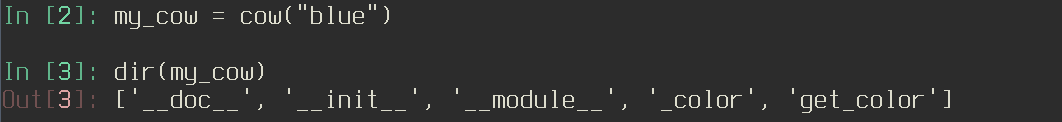
\includegraphics[scale=0.35]{medias/api_discover.png}
\end{frame}

\begin{frame}
  \frametitle{IPython - Utile pour \ldots}
    \begin{itemize}
      \item embarquer un shell IPython dans ses programmes
    \end{itemize}
  
\includegraphics[scale=0.35]{medias/embedded_ipython.png}
\end{frame}
\newpage


\section{Les types de base de Python}
\subsection{Quelques types simples}
% 1 Les types de base Python
% 1.1 Quelques types simples
%     - entiers
%     - les réels (flottants)
%     - les complexes
%     - les booléens (True, False)
%     - le type None

\begin{frame}
  \frametitle{Quelques types simples}
  \begin{itemize}
    \item<1-> les entiers
    \item<2-> les flottants
    \item<3-> les complexes
    \item<4-> les booléens
    \item<5-> la valeur 'Rien'
  \end{itemize}
\end{frame}

\begin{frame}[fragile]
  \frametitle{Quelques types simples}
  \begin{itemize}
    \item les entiers
  \end{itemize}
\begin{ipython}
\ipinpt{my_int = 12}
\ipinpt{my_other_int = int("12")}
\ipinpt{my_int + my_other_int}
\ipoutp{24}
\end{ipython}
\end{frame}

\begin{frame}[fragile]
  \frametitle{Quelques types simples}
  \begin{itemize}
    \item les flottants
  \end{itemize}
\begin{ipython}
\ipinpt{my_float = 3.14}
\ipinpt{print float(42)}
\ipoutp{42.0}
\ipinpt{print 2/5}
\ipoutp{0}
\ipinpt{print 2/5.0}
\ipoutp{0.40000000000000002}
\end{ipython}
\end{frame}

\begin{frame}[fragile]
  \frametitle{Quelques types simples}
  \begin{itemize}
    \item les complexes
  \end{itemize}
\begin{ipython}
\ipinpt{my_cplx = 5+2j}
\ipinpt{my_cplx.real}
\ipoutp{5.0}
\ipinpt{my_cplx.imag}
\ipoutp{2.0}
\ipinpt{my_cplx.conjugate()}
\ipoutp{(5-2j)}
\ipinpt{abs(my_cplx)}
\ipoutp{5.3851648071345037}
\end{ipython}
\end{frame}

\begin{frame}[fragile]
  \frametitle{Quelques types simples}
  \begin{itemize}
    \item les booléens : \alert{True, False}
    \item la valeur 'Rien' : \alert{None}
  \end{itemize}
\begin{ipython}
\ipinpt{print True | False}
\ipoutp{True}
\ipinpt{print True and False}
\ipoutp{False}
\ipinpt{print type(None)}
\ipoutp{<type 'NoneType'>}
\end{ipython}
\end{frame}

% 1.2 Quelques structures de données
%     - les chaines de caractère sont des séquences comme les autres mais sont différentes dans la tête des gens
%     - séquence: list modifiable, tuple non modifiable, queue...
%     - dictionnaire
%     - ensemble (partie gauche d'un dict): set modifiable, frozenset non modifiable

\subsection{Quelques structures de données}
\begin{frame}
  \frametitle{Quelques structures de données}
  \begin{itemize}
    \item<1-> les chaînes de caractère, un cas particulier de séquence
    \item<2-> les autres séquences : tuples, listes \ldots
    \item<3-> les dictionnaires
    \item<4-> les sets, frozenset
  \end{itemize}
\end{frame}

\begin{frame}[fragile]
\frametitle{Quelques structures de données}
\begin{itemize}
\item Généralités sur les séquences (liste, tuple, chaînes)
\end{itemize}
\begin{ipython}
\ipinpt{sequence = [1,2,3,4] \#liste pour exemple}
\ipinpt{print sequence[1]}
\ipoutp{2}
\ipinpt{print sequence[:3]}
\ipoutp{[1,2,3]}
\ipinpt{print sequence[-1]}
\ipoutp{4}
\end{ipython}
\end{frame}

\begin{frame}[fragile]
  \frametitle{Quelques structures de données}
  \begin{itemize}
    \item les chaînes de caractères
  \end{itemize}
\begin{ipython}
\ipinpt{my\_str = "hello"}
\ipinpt{my\_other\_str = 'hello'}
\ipinpt{my\_third\_str = """My}
\ipcont{tailor is}
\ipcont{rich."""}
\ipinpt{my\_last\_str = str(42)}
\ipinpt{my\_last\_str + my\_str}
\ipoutp{42hello}
\end{ipython}
\end{frame}

\begin{frame}[fragile]
  \frametitle{Quelques structures de données}
    \begin{itemize}
    \item manipulation de chaîne de caractères
    \end{itemize}
\begin{ipython}
\ipinpt{a = "une string"}
\ipinpt{print(a.split(' '))}
\ipoutp{['une', 'string']}
\ipinpt{print a.upper()}
\ipoutp{UNE STRING}
\end{ipython}
\end{frame}

\begin{frame}[fragile]
  \frametitle{Quelques structures de données}
  \begin{itemize}
    \item les listes
  \end{itemize}
  \begin{ipython}
\ipinpt{my\_str = "cardboard"}
\ipinpt{my\_list = [1, my\_str, (2, 3, 4)]}
\ipinpt{my\_list.append(321)}
\ipinpt{print my\_list}
\ipoutp{[1, 'cardboard', (2, 3, 4), 321]}
\ipinpt{my\_list.extend([2,3])}
\ipinpt{print my\_list}
\ipoutp{[1, 'cardboard', (2, 3, 4), 321, 2, 3]}
  \end{ipython}
\end{frame}

\begin{frame}[fragile]
  \frametitle{Quelques structures de données}
    \begin{itemize}
      \item les tuples (séquences non éditables)
    \end{itemize}
\begin{ipython}
\ipinpt{my\_tuple = (1, 1, "hello", 1, 1.5)}
\ipinpt{print my\_tuple.count(1)}
\ipoutp{3}
\ipinpt{my\_other\_tuple = tuple("epsilon")}
\ipinpt{my\_other\_tuple}
\ipoutp{('e', 'p', 's', 'i', 'l', 'o', 'n')}
\end{ipython}
\end{frame}

\begin{frame}[fragile]
  \frametitle{Quelques structures de données}
  \begin{itemize}
    \item les dictionnaires (tableaux associatifs)
  \end{itemize}
  \begin{ipython}
\ipinpt{my\_dict = \{"key1":"value1", }
\ipcont{           "key2":"value2"\}}
\ipinpt{my\_dict["key3"] = "value3"}
\ipinpt{my\_dict["key2"]}
\ipoutp{'value2'}
\ipinpt{my\_dict.keys()}
\ipoutp{['key3', 'key2', 'key1']}
\ipinpt{my\_dict.items()}
\ipoutp{[('key3', 'value3'), ('key2', 'value2'),}
\ipwrapp{('key1', 'value1')]}
  \end{ipython}
\end{frame}

\begin{frame}[fragile]
  \frametitle{Quelques structures de données}
  \begin{itemize}
    \item Les sets assurent l'unicité de leurs éléments
    \item Les sets permettent des opérations ensemblistes (union, différence symétrique)
    \item Seuls des éléments 'hashable' peuvent être insérés dans les sets
    \item Les frozensets sont aux sets ce que le tuple est au liste (non éditable)
  \end{itemize}
\end{frame}

\begin{frame}[fragile]
  \frametitle{Quelques structures de données}
  \begin{ipython}
\ipinpt{my\_set = set(["blue", "green", "green"])}
\ipinpt{my\_set.add("yellow")}
\ipinpt{my\_set}
\ipoutp{set(['blue', 'green', 'yellow'])}
\ipinpt{my\_set.add("yellow")}
\ipinpt{my\_set}
\ipoutp{set(['blue', 'green', 'yellow']])}
\ipinpt{my\_other\_set = set(("green", "rogen"))}
\ipinpt{my\_set.intersection(my\_other\_set)}
\ipoutp{set(['green'])}
  \end{ipython}
\end{frame}

% 1.3 Quelques autres types courants (juste les évoquer)
%     - classe, fonction ou méthode, module...

\subsection{Quelques autres types courants}
\begin{frame}
  \frametitle{Quelques autres types courants}
  \begin{itemize}
    \item les classes
    \item les fonctions/méthodes
    \item les modules
  \end{itemize}
\end{frame}

% 2 La syntaxe de Python
% 2.1 instructions
%     - séparateur d'instruction : ';' (éviter) ou '\\n'
% 2.2 blocs
%     - contexte (scope) défini par bloc
%     - blocs définis par :
%       - leur niveau d'indentation
%       - bloc de niveau inférieur suit une ligne
%         - qui commence par un mot clef (if, while, for, def, class, with)
%         - se termine par ':'
% et continuer comme julien l'a fait sur if etc.
% Ce point 2.2 est une introduction aux différents blocs qu'on va traiter ensuite.


\section{La grammaire de Python}

\subsection{Les variables}
\begin{frame}[fragile]
  \frametitle{Les variables}
  \begin{itemize}
  \item La déclaration d'une variable est implicite
  \item Le typage en python est automatique
  \end{itemize}
  \begin{ipython}
  \ipinpt{x = 2}
  \ipinpt{type(x)}
  \ipoutp{print <type 'int'>}
  \ipinpt{x = "x est désormais une string"}
  \ipinpt{print type(x)}
  \ipoutp{<type 'str'>}
  \end{ipython}
\end{frame}


\subsection{Les blocs de code}
\begin{frame}[fragile]
  \frametitle{Les blocs de code, ou suites}
  \begin{description}
  \item[L'indentation du code] est par convention un multiple de 4 espaces. \pause
  \item[Un bloc de code] est constitué de lignes de code dont le niveau d'indentation/d'imbrication est égal ou supérieur à celui de sa première ligne. \pause
  \item[Des sous-blocs] sont donc éventuellement présents au sein d'un bloc de code, en tant que membres d'instructions composées.
  \end{description}
\end{frame}

\subsection{Les instructions composées}
\subsubsection{Définition}
\begin{frame}[fragile]
  \frametitle{Les instructions composées : définition}
  \begin{description}
  \item[Les instructions composées] sont introduites par une instruction elle-même composée \pause
  \begin{itemize}
      \item d'un mot clef parmi «\hlcmd{if}», «\hlcmd{for}», «\hlcmd{def}»~\ldots \pause
      \item suivi par des paramètres \pause
      \item conclue par «\hlcmd{:}» \pause
  \end{itemize}
  \item[Un ou plusieurs blocs d'instruction] sont contenus dans une instruction composée.
  \end{description}
\end{frame}

\subsubsection{Exemple}
\begin{frame}[fragile]
  \frametitle{Les instructions composées : l'exemple de if}
  \emph{Le «\texttt{if}» tel que dans la grammaire:}\\
  \begin{beamercolorbox}{documentation}
  \small{\verb|if_stmt:|} \\
  \small{\verb|    'if' test ':' suite|} \\
  \small{\verb|    ('elif' test ':' suite)*|} \\
  \small{\verb|    ['else' ':' suite]|}
  \end{beamercolorbox}
\end{frame}

\begin{frame}[fragile]
  \frametitle{Les instructions composées : l'exemple de if}
  \begin{ipython}
  \ipinpt{if 2 + 2 == 5 :}
  \ipcont{    print "2 est grand"}
  \ipcont{elif 1 > 1:}
  \ipcont{    print "1 s'est toujours",}
  \ipcont{    print "cru supérieur."}
  \ipcont{else:}
  \ipcont{    print "Un monde banal",}
  \ipcont{    print "et ennuyeux. "}
  \ipcont{...}
  \ipcont{...}
  \ipoutp{Un monde banal et ennuyeux.}
  \end{ipython}
\end{frame}

\subsubsection{Liste brute}
\begin{frame}[fragile]
  \frametitle{Les instructions composées : liste}
Liste fournie pour référence, ne pas essayer de tout comprendre maintenant !
\end{frame}

\begin{frame}[fragile]
  \frametitle{Les instructions composées : liste brute}
\begin{figure}
  \begin{beamercolorbox}{documentation}
\scriptsize\begin{verbatim}
if_stmt: 'if' test ':' suite ('elif' test ':' suite)* ['else' ':' suite]
while_stmt: 'while' test ':' suite ['else' ':' suite]
for_stmt: 'for' exprlist 'in' testlist ':' suite ['else' ':' suite]
try_stmt: ('try' ':' suite
           ((except_clause ':' suite)+
            ['else' ':' suite]
            ['finally' ':' suite] |
           'finally' ':' suite))
with_stmt: 'with' with_item (',' with_item)*  ':' suite
with_item: test ['as' expr]
# NB compile.c makes sure that the default except clause is last
except_clause: 'except' [test [('as' | ',') test]]
\end{verbatim}
  \end{beamercolorbox}
\def\figurename{extrait de la grammaire de Python}
\caption{http://docs.python.org/reference/grammar.html}
\end{figure}
\end{frame}

\begin{frame}[fragile]
  \frametitle{Les instructions composées : liste traduite}
Soit grosso modo, en français
\small\begin{tabular}{|l|l|l|}
\hline
mot clef & rôle & suivi de / variante \\
\hline \hline
\texttt{if} & condition & suivi de \texttt{0..* elif}, \texttt{0..1 else}\\ \hline
\texttt{while} & boucle "tant que" & suivi de \texttt{0..1 else}\\ \hline
\texttt{for} & itération sur éléments & suivi de \texttt{0..1 else}\\ \hline
\texttt{try} & fournit un mécanisme & suivi de \texttt{finally}\\
 & de gestion des &  ou de \texttt{1..* except}, \\
 & exceptions & \texttt{0..1 finally}, \texttt{0..1 else}\\ \hline
\texttt{with} & définition de contexte & \\ \hline
\texttt{def} & définition de fonction & variante décorée \\ \hline
\texttt{class} & définition de classe & variante décorée \\ \hline
\end{tabular}
\end{frame}


\begin{frame}[fragile]
  \frametitle{Déclarations composées : exemple d'imbrication}
\begin{figure}
\tiny{\begin{lstlisting}import sys
from PyQt4.QtGui import QApplication
from gitbuster.main_window import MainWindow, \
                         select_git_directory
def main():
    app = QApplication(sys.argv)
    filepath = select_git_directory()
    if filepath:
        a = MainWindow(directory=filepath, debug=True)
        a.show()
        sys.exit(app.exec_())
    else:
        sys.exit(1)
  \end{lstlisting}}
\def\figurename{Code source de gitbuster}
\caption{https://github.com/mike-perdide/gitbuster}
\end{figure}
\end{frame}

\subsection{Les instructions}
\begin{frame}
  \frametitle{Syntaxe - Les instructions}
  \begin{itemize}
    \item<1-> Au sein d'un bloc, on sépare généralement chaque instruction par un retour à la ligne.
    \item<2-> La ligne suivante, si elle fait partie du même bloc, doit avoir la même indentation.
    \item<3-> Il est aussi possible, bien que déconseillé, de mettre plusieurs instructions sur une ligne
    \begin{itemize}
      \item<4-> Il faut alors les séparer par ';'
    \end{itemize}
  \end{itemize}
\end{frame}

\subsection{Les instructions conditionnelles}
\begin{frame}[fragile]
  \frametitle{Déclarations conditionnelles - Syntaxe de base}
  \begin{lstlisting}
if condition1:
    declaration1
elif condition2:
    declaration2
else:
    declaration3
  \end{lstlisting}
\end{frame}

\begin{frame}[fragile]
  \frametitle{Déclarations conditionnelles - Exemple}
  \begin{lstlisting}
my_str = "word"
if 1 > 2:
    print "1>2"
elif my_str == "word":
    print "my_str = word"
else:
    print "else"
  \end{lstlisting}

  \begin{beamercolorbox}{terminal}
  \begin{semiverbatim}
 \$ python example.py
 \uncover<2>{my_str = word} \end{semiverbatim}
  \end{beamercolorbox}

\end{frame}

\begin{frame}[fragile]
  \frametitle{Syntaxe - Les conditions}
  \begin{itemize}
    \item les comparaisons
  \end{itemize}
  \begin{ipython}
    \ipinpt{(1 == 2, 1 < 2, 2 < 1, 1 != 2)}
    \ipoutp{(False, True, False, True)}
    \ipinpt{my_str = "hello"}
    \ipinpt{(my_str == "hello",}
    \ipcont{ my_str > "helln", }
    \ipcont{ my_str < "hellq") }
    \ipoutp{(True, True, True)}
  \end{ipython}
\end{frame}

\begin{frame}[fragile]
  \frametitle{Syntaxe - Les conditions}
  \begin{itemize}
    \item les opérateurs booléens
  \end{itemize}
  \begin{ipython}
    \ipinpt{not True and False or not False}
    \ipoutp{True}
  \end{ipython}
\end{frame}

\begin{frame}[fragile]
  \frametitle{Syntaxe - Les conditions}
  \begin{itemize}
    \item par extension, certains objets vides sont équivalent à False
  \end{itemize}
  \begin{ipython}
    \ipinpt{my_str = ""}
    \ipinpt{if not my_str:}
    \ipcont{    print "False"}
    \ipoutp{False}
  \end{ipython}
\end{frame}

\subsection{Les boucles}
\begin{frame}[fragile]
  \frametitle{Syntaxe - Les boucles}
  \begin{itemize}
    \item for : répéter tant qu'il y a des éléments dans un ensemble
    \item while : répéter tant qu'une condition reste vraie
  \end{itemize}

  Compatible : break/continue (comme dans les autres langages)
\end{frame}

\begin{frame}[fragile]
  \frametitle{Syntaxe de for}
  \begin{lstlisting}
for item in <generator>:
    code ...
  \end{lstlisting}
Examples de générateur :
  \begin{itemize}
  \item ("item1", "item2", "item3")
  \item range(5) ou (0, 1, 2, 3, 4)
  \item xrange(5)
  \item n'importe quel objet ayant la méthode next()
  \end{itemize}
\end{frame}

\subsection{Les méthodes/fonctions}
\begin{frame}[fragile]
  \frametitle{Syntaxe - Les méthodes/fonctions}
  \begin{itemize}
    \item En Python, la signature d'une méthode n'inclut pas le type retourné.
    \item Les arguments passés peuvent être des paramètres et/ou des arguments nommés.
    \item Le mot clef utilisé est {\bf def}.
    \item TODO: parler des scopes. cf http://www.network-theory.co.uk/docs/pytut/PythonScopesandNameSpaces.html
  \end{itemize}
\end{frame}

\begin{frame}[fragile]
  \frametitle{Syntaxe de def}
Avec des paramètres :
  \begin{lstlisting}
def nom_de_methode(arg1, arg2, arg3):
    code ...
  \end{lstlisting}
Avec des arguments nommés :
  \begin{lstlisting}
def nom_de_methode(arg1=True, arg2=3):
    code ...
  \end{lstlisting}
Fonction variadique :
  \begin{lstlisting}
def nom_de_methode(*args, **kwargs):
    code ...
  \end{lstlisting}
\end{frame}

\begin{frame}[fragile]
  \frametitle{Fonctions - Valeur de retour}
Pour que la fonction retourne une valeur, il faut utiliser le mot clef {\bf return}.
  \begin{lstlisting}
def nom_de_methode(arg1, arg2, arg3):
    code ...
    return value
  \end{lstlisting}

La signature n'incluant pas le type retourné, il est possible de retourner des types d'objets différents selon les contextes d'utilisation, mais dans la pratique c'est une mauvaise idée.
\end{frame}

\subsection{Les classes}
\begin{frame}[fragile]
  \frametitle{Syntaxe - Les classes}
  \begin{itemize}
    \item<1-> Python, langage orienté objet, permet la définition de nouveaux types d'objets grâce au mot clef {\bf class}.
    \item<2-> Les classes comportent une méthode \verb=__init__= ("constructeur").
    \item<3-> Toutes les méthodes d'une classes prennent pour premier argument \verb=self= (par convention).
    \begin{itemize}
      \item<3-> \verb=self= est l'objet sur lequel est appelé la méthode.
    \end{itemize}
    \item<4-> Les classes peuvent dériver de classes parentes et hériter de leurs attributs.
  \end{itemize}
\end{frame}

\begin{frame}[fragile]
  \frametitle{Syntaxe de class}
  \begin{lstlisting}
class nom_de_classe(classe_parente):
    def __init__(self, arg1):
        classe_parente.__init__(self)

        self._attr1 = arg1

    def methode_1(self, arg1):
        code...
  \end{lstlisting}
\end{frame}

\section{Autre}
% ici: des infos sur les namespaces, les objets


\section{Quelques librairies standard}
\begin{frame}[fragile]
  \frametitle{Quelques librairies standard}
  \begin{itemize}
    \item<1-> {\bf subprocess}, la gestion des process
    \item<2-> {\bf socket}, pour la communication réseau
    \item<3-> {\bf os}, interaction avec le système hôte
    \item<4-> {\bf threading}, pour les threads
  \end{itemize}
\end{frame}



\end{document}
